\documentclass[12pt]{report}

\usepackage{amssymb, fullpage, amsmath,esint}
\usepackage{graphicx}

\newtheorem{problem}{Problem}

\newenvironment{solution}[1][\it{Solution}]{\textbf{#1. } }{$\square$}

\graphicspath{ {./} }

\allowdisplaybreaks

\pagestyle{empty}

\def\Z{{\mathbb Z}}
\def\Q{{\mathbb Q}}
\def\C{{\mathbb C}}
\def\R{{\mathbb R}}
\def\N{{\mathbb N}}
\def\eps{{\epsilon}}
\def\O{{\mathcal{O}}}
\newcommand{\floor}[1]{{\left\lfloor#1\right\rfloor}} % Floor function
\newcommand{\ceil}[1]{{\left\lceil#1\right\rceil}} % Ceiling function
\newcommand{\paren}[1]{{\left(#1\right)}} % Parentheses ()
\newcommand{\brac}[1]{{\left\{#1\right\}}} % Curly braces {}
\newcommand{\braces}[1]{{\left[#1\right]}} % Braces []
\newcommand{\abrac}[1]{{\left\langle#1\right\rangle}} % Angle Braces <>
\newcommand{\abs}[1]{{\left|#1\right|}} % Absolute value
\newcommand{\norm}[1]{{\left\|#1\right\|}} % Norm
\newcommand{\eval}[2]{\right|_{#1}^{#2}} % Evaluate

\newcommand{\pp}[2]{\frac{\partial #1}{\partial #2}} % Partial of 1 wrt 2
\newcommand{\ppn}[3]{\frac{\partial^{#1} #2}{\partial #3^{#1}}} % nth Partial of 1 wrt 2
\newcommand{\dd}[2]{\frac{\mathrm{d} #1}{\mathrm{d} #2}} % Partial of 1 wrt 2
\newcommand{\ddn}[3]{\frac{\mathrm{d}^{#1} #2}{\mathrm{d} #3^{#1}}} % nth Partial of 1 wrt 2

\def\Xint#1{\mathchoice
   {\XXint\displaystyle\textstyle{#1}}%
   {\XXint\textstyle\scriptstyle{#1}}%
   {\XXint\scriptstyle\scriptscriptstyle{#1}}%
   {\XXint\scriptscriptstyle\scriptscriptstyle{#1}}%
   \!\int}
\def\XXint#1#2#3{{\setbox0=\hbox{$#1{#2#3}{\int}$}
     \vcenter{\hbox{$#2#3$}}\kern-.5\wd0}}
\def\ddashint{\Xint=}
\def\dashint{\Xint-}
\def\ointcc{{\ointctrclockwise}}
\def\ointc{{\ointclockwise}}

\begin{document}

\large

\begin{center}
 Math 567 Homework 4\\
 Due October 27\\
 By Marvyn Bailly\\
\end{center}

\normalsize

\hrule

%---------------%
%---Problem 1---%
%---------------%

%--status--$

\begin{problem}
    Using residue calculus, calculate
    \[ I = \int_{-\infty}^{\infty} \frac{\sin(x)}{\sinh{x}} dx.\]
\end{problem}

\begin{solution}
    
    \noindent
    To evaluate the real integral,
    \[
        I = \int_{-\infty}^{\infty} \frac{\sin(x)}{\sinh{x}} dx = \dashint_{-\infty}^{\infty} \frac{\sin(x)}{\sinh{x}} dx,
    \]
    we will consider the integral in the complex plane with,
    \[
        \ointcc_C \frac{\sin(z)}{\sinh{z}} dz = \paren{\int_{C_1} + \int_{C_R} + \int_{C_2} + \int_{C_\epsilon} + \int_{C_3} + \int_{C_L}}\frac{\sin(z)}{\sinh{z}} dz,
    \]
    where $C$ is the contour described in the following figure.
    \begin{center}
        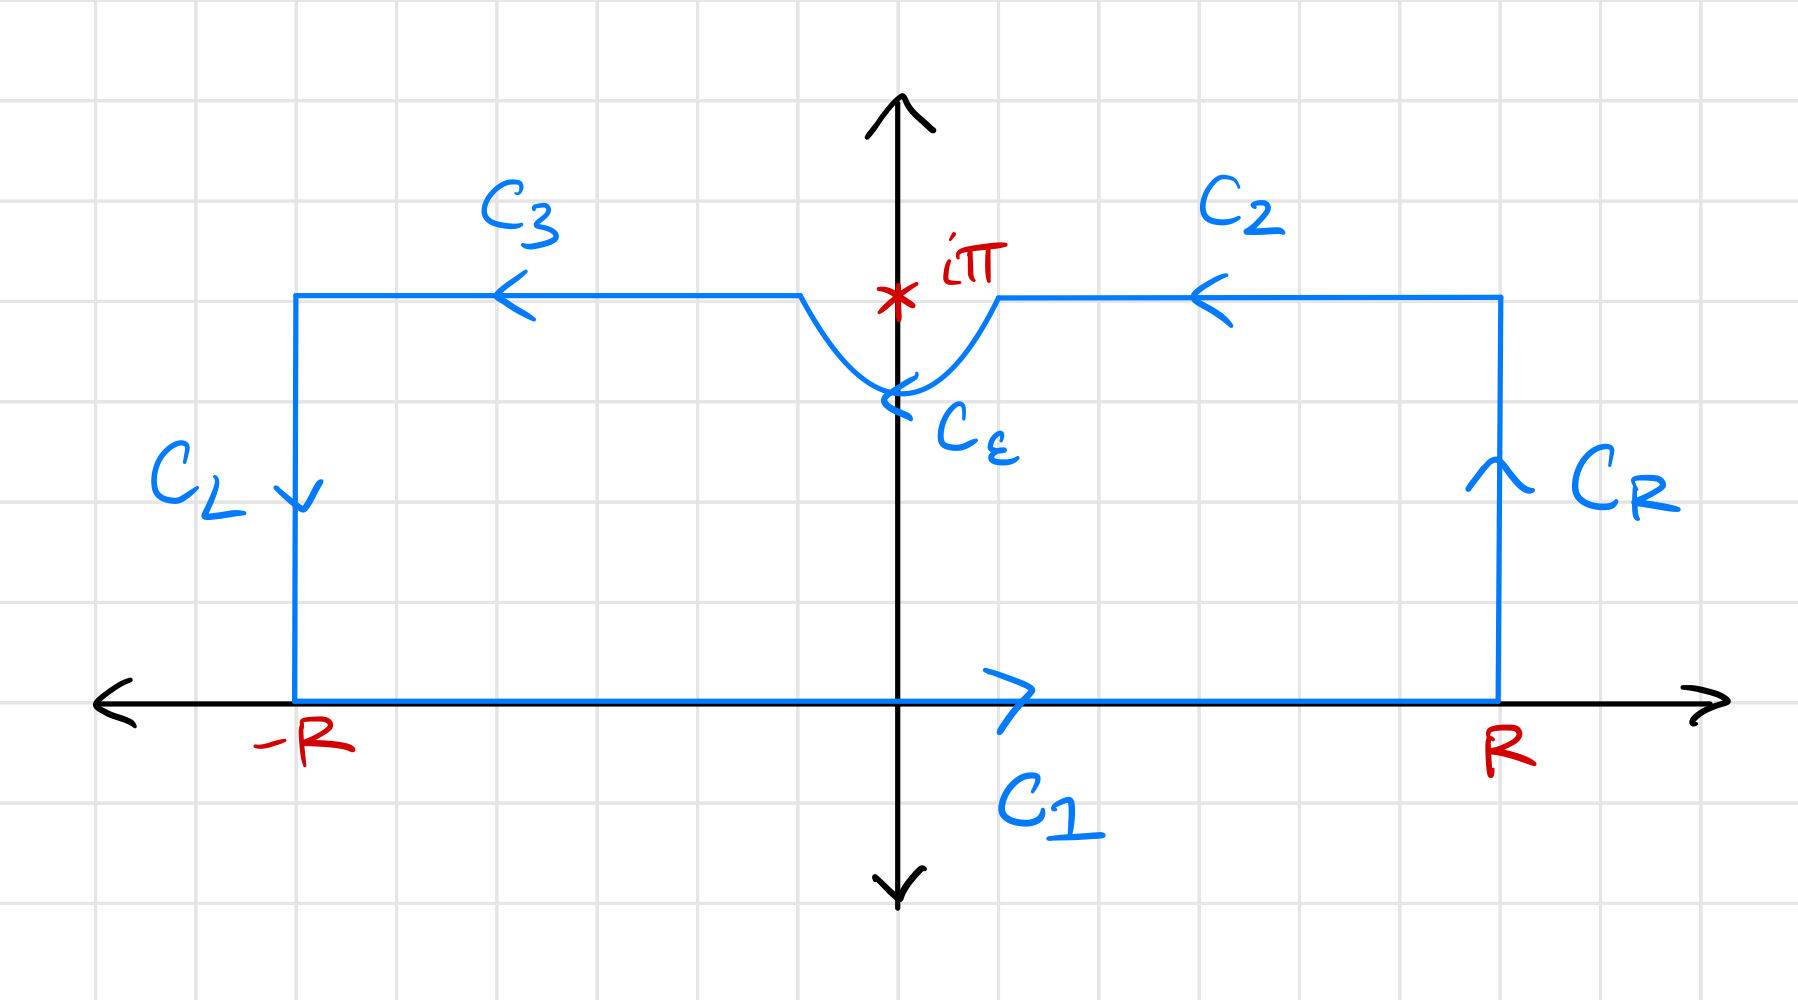
\includegraphics[width=.5\textwidth]{fig1.png}
    \end{center}
    We know that the function is analytic on and inside $C$ without the discontinuity at $z = 0$, we have that 
    \[ 
        \ointcc_C \frac{\sin(z)}{\sinh{z}} dz = 0,
    \]
    by Cauchy's Theorem. Next consider $C_R$,
    \[ 
        \int_{C_R} \frac{\sin(z)}{\sinh{z}} = \int_{0}^{\pi} \frac{\sin(R + iy)}{\sinh{(R + iy)}}idy = \int_{0}^{\pi} \frac{e^{iR}e^{-y} - e^{-iR}e^{y}}{e^Re^{iy} - e^{-R}e^{-iy}}dy.
    \]
    And since,
    \begin{align*}
        \lim_{R \rightarrow \infty} \abs{\frac{e^{iR}e^{-y} - e^{-iR}e^{y}}{e^Re^{iy} - e^{-R}e^{-iy}}} 
        &\leq \lim_{R \rightarrow \infty} \frac{\abs{e^{iR}}\abs{e^{-y}} + \abs{e^{-iR}}\abs{e^{y}}}{\abs{\abs{e^R}\abs{e^{iy}} - \abs{e^{-R}}\abs{e^{-iy}}}}\\
        &= \lim_{R \to \infty} \frac{e^{-y} + e^y}{\abs{e^R - e^{-R}}}\\
        &= 0,
    \end{align*}
    for $0\leq y \leq \pi$. Thus we have that,
    \[ 
        \lim_{R \to \infty} \int_{C_R} \frac{\sin(z)}{\sinh(z)}dz = 0.
    \]
    Next notice that $C_L$,
    \[ 
        \int_{C_L} \frac{\sin(z)}{\sinh(z)}dz = \int_{\pi}^{0} \frac{\sin(-R + iy)}{\sinh(-R + iy)} = \int_{\pi}^{0} \frac{e^{iR}e^{-y} - e^{iR}e^{y}}{e^{-R}e^{iy} - e^{R}e^{-iy}}dy.
    \]
    Since
    \begin{align*}
        \lim_{R \to \infty} \abs{\frac{e^{iR}e^{-y} - e^{iR}e^{y}}{e^{-R}e^{iy} - e^{R}e^{-iy}} } &\leq \lim_{R \to \infty} \frac{\abs{e^{iR}}\abs{e^{-y}} + \abs{e^{iR}}\abs{e^{y}}}{\abs{\abs{e^{-R}}\abs{e^{iy}} - \abs{e^{R}}\abs{e^{-iy}}}}\\
        &= \lim_{R \to \infty} \frac{e^{-y} + e^y}{\abs{e^{-R} - e^R}}\\
        &= 0,
    \end{align*}
    for $0 \leq y \leq \pi$ we have shown that,
    \[ 
        \int_{C_L} \frac{\sin(z)}{\sinh(z)}dz = 0.
    \]
    We have a simple pole at $z = i\pi$,
    \[
        \int_{C_\epsilon} \frac{\sin(z)}{\sinh{z}} dz = -i \pi \text{Res}(i\pi) = -i\pi \paren{\frac{\sin(i\pi)}{\cosh(i\pi)}} = -i\pi \paren{\frac{i\sinh(\pi)}{\cos(\pi)}} = -\pi \sinh(\pi).
    \]
    Now let's look at,
    \[ 
        \paren{\int_{C_2} + \int_{C_3}} \frac{\sin(z)}{\sinh(z)}dz = \dashint_{R}^{-R} \frac{\sin(x + i\pi)}{\sinh(x + i\pi)}dx.
    \]
    Observe that,
    \begin{align*}
        \frac{\sin(x + i\pi)}{\sinh(x + i\pi)} &= \frac{\sin(x)\cos(i\pi) + \sin(i\pi)\cos(x)}{\sinh(x)\cosh(i\pi) + \sinh(i\pi)\cosh(x)}\\
        &= \frac{\sin(x)\cosh(\pi) + i\sinh(\pi)\cos(x)}{\sinh(x)\cos(\pi) + i\sin(\pi)\cosh(x)}\\
        &= -\cosh(\pi) \paren{\frac{\sin(x)}{\sinh(x)}} - i\sinh(\pi)\paren{\frac{\cos(x)}{\sinh(x)}}.
    \end{align*}
    We know that $\frac{\cos(x)}{\sinh(x)}$ is an odd function. Using this fact we can rewrite the integral as,
    \[ \lim_{R \to \infty} \paren{\int_{C_2} + \int_{C_3}}\frac{\sin(z)}{\sinh(z)}dz = -\cosh(\pi) \lim_{R \to \infty} \dashint_{R}^{-R}dx = \cosh(\pi) I.\]
    And since,
    \[ \lim_{R \to \infty} \int_{C_1} \frac{\sin(z)}{\sinh(z)}dz = \lim_{R \to \infty} \int_{-R}^{R} \frac{\sin(x)}{\sinh{x}} dx = I.\]
    Thus we that,
    \[ 0 = -\pi \sinh(\pi) + I + \cosh(\pi) I,\]
    and so we have that,
    \[ I = \pi \paren{\frac{\sinh(\pi)}{1 + \cosh(\pi)}} = \pi \tanh\paren{\frac{\pi}{2}}.\]
\end{solution}

%----------------------------------------------------------------------------------------------------%
%\vskip 20pt
\newpage

%---------------%
%---Problem 2---%
%---------------%

%--status--$

\begin{problem}
    Use Residue calculus, calculate
    \[
        I = \int_{-\infty}^{\infty} \frac{1 + \cos{x}}{(x - \pi)^2}dx.
    \]
\end{problem}

\begin{solution}
    
    \noindent
    Consider the integral,
    \[ 
        I = \int_{-\infty}^{\infty} \frac{1 + \cos(x)}{(x - \pi)^2}dx = \int_{-\infty}^{\infty} \frac{1 - \cos(x)}{x^2}dx,
    \]
    since $\cos(x - \pi) = -\cos(x)$. Then,
    \[ 
        I = \int_{-\infty}^{\infty} = \frac{1 - \cos(x)}{x^2}dx = \dashint_{-\infty}^{\infty} \frac{1 - \cos(x)}{x^2}dx.
    \] 
    Now consider the integral in the complex plane,
    \begin{align*}
        \text{P} \ointcc_C \frac{1 - \cos(x)}{x^2}dx &= \text{Re}\paren{\text{P}\int_{-\infty}^{\infty} \frac{1 - e^iz}{z^2}dz}\\
        &= \text{Re}\paren{\text{P}\int_{-\infty}^{\infty} \frac{e^{i0z} - e^iz}{z^2}dz},
    \end{align*}
    where $C$ is the closed semicircular sector in the upper half plane from $R$ to $-R$. Now Observe that,
    \begin{align*}
        \lim_{R \to \infty} \abs{ \frac{1}{z^2}} &= \lim_{R \to \infty} \frac{1}{|z^2|}\\
        &= \lim_{R \to \infty} \frac{1}{|R^2||e^{i2\theta}|}\\
        &= \lim_{R \to \infty} \frac{1}{R^2}\\
        &= 0.
    \end{align*}
    So we can apply Jordan's Lemma,
    \begin{align*}
        \text{P}\int_{-\infty}^{\infty} \frac{e^{i0z} - e^iz}{z^2}dz = \dashint_{-\infty}^{\infty} \frac{1 - \cos(x)}{x^2}dx.
    \end{align*}
    Now consider that since there is a simpler pole at $z=0$, it must be that,
    \begin{align*}
        \dashint_{-\infty}^{\infty} \frac{1 - \cos(x)}{x^2}dx &= i\pi \text{Res}(0)\\
        &= i\pi \paren{\lim_{z \to 0} \frac{1 - e^{iz}}{z}}\\
        &= i \pi \paren{\lim_{z \to 0} \frac{-iz + \O(z^2)}{z}}\\
        &= i \pi \paren{\lim_{z \to 0} -i + \O(z)}\\
        &= \pi.
    \end{align*}
    Therefore we have that,
    \begin{align*}
        I = \dashint_{-\infty}^{\infty} \frac{1 - \cos(x)}{x^2}dx &= \text{Re}\paren{\dashint_{-\infty}^{\infty} \frac{1 - e^{iz}}{z^2}}\\
        &= \text{Re}\paren{P \ointcc_{-\infty}^{\infty} \frac{e^{i0z} - e^{iz}}{z^2}dz}\\
        &=\pi.
    \end{align*}
\end{solution}

%----------------------------------------------------------------------------------------------------%
%\vskip 20pt
\newpage

%---------------%
%---Problem 3---%
%---------------%

%--status--$

\begin{problem}
    Evaluate the following integral using residue calculus,
    \[ 
        I = \int_0^\infty \frac{x^a}{1 + 2x \cos(b) + x^2}dx,
    \]
    where $-1< a < 1, a\neq 0$ and $-\pi \le b \le \pi, b\neq 0.$ 
\end{problem}

\begin{solution}

    \noindent
    Consider the integral
    \begin{align*}
        I &= \int_0^\infty \frac{x^a}{1 + 2x \cos(b) + x^2}dx\\
        &= \int_0^\infty \frac{x^a}{(x + \cos(b) + i\sin(b))(x + \cos(b) - i\sin(b))}dx\\
        &= \int_0^\infty \frac{x^a}{(x + e^{ib})(x + e^{-ib})}dx,
    \end{align*} 
    where $-1< a < 1, a\neq 0$ and $-\pi \le b \le \pi, b\neq 0.$
    Now let's consider this integral in the complex plane
    \[ 
        \ointcc_C \frac{z^a}{(z + e^{ib})(z + e^{-ib})}dz = \paren{\int_{C_1} + \int_{C_R} + \int_{C_2} + \int_{C_\rho}}\frac{z^a}{(z + e^{ib})(z + e^{-ib})}dz,
    \]
    where $0 \leq \arg(z) \le 2\pi$ is the necessary branch cut to make our $x^a$ single valued and $C$ is the contour described in the figure kindly drawn by Rohin.
    \begin{center}
        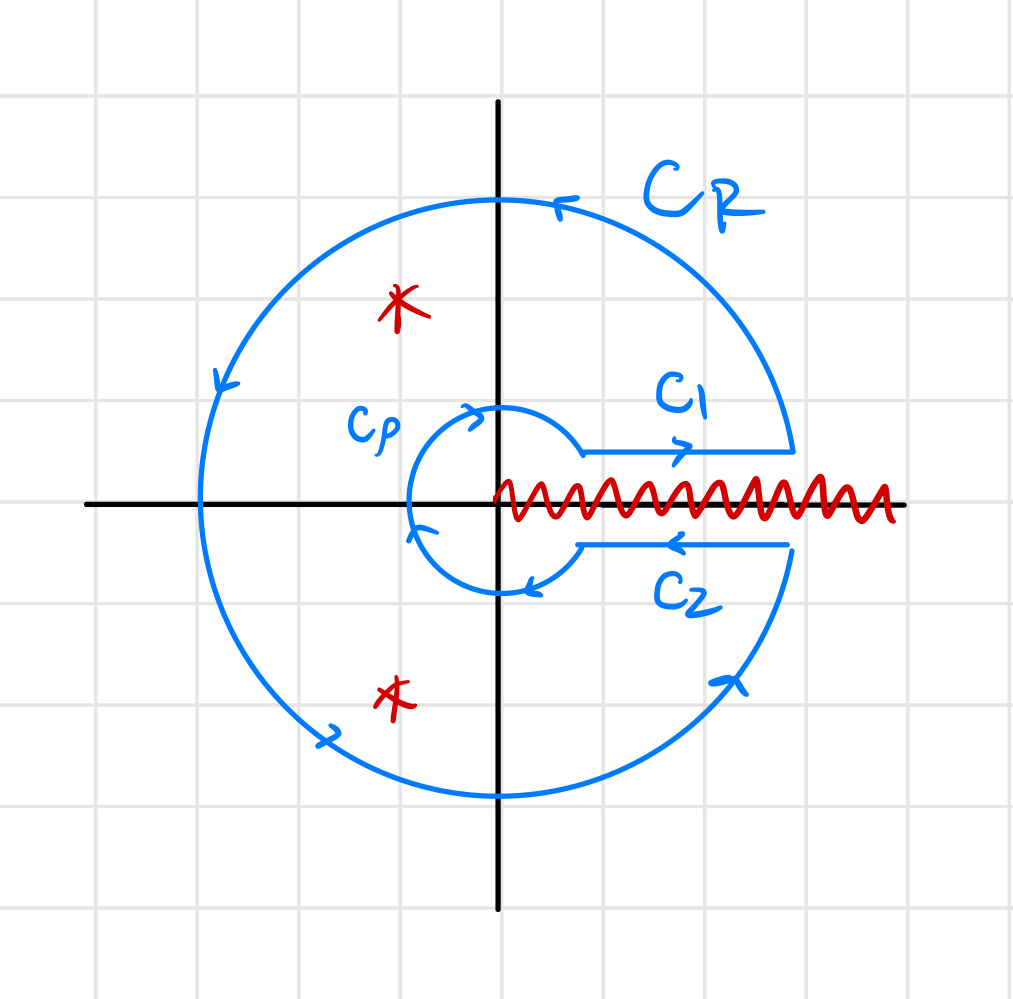
\includegraphics[width=.5\textwidth]{fig2.png}
    \end{center}
    Note the two poles at $z= -e^{\pm ib}$ which can be rewritten as 
    \[
        -e^{ib} = e^{ib}e^{i\pi} = e^{i(b + \pi)}, ~~~ \text{and} ~~~ -e^{-ib} = e^{-ib}e^{\pi} = e^{i(-b + i)},
    \]
    which are within the contour. 
    Since the function is analytic on and within $C$, we can apply Residue theorem
    \begin{align*}
        \ointcc_C \frac{z^a}{(z + e^{ib})(z + e^{-ib})}dz &= 2\pi i \paren{\text{Res}(-e^{ib}) + \text{Res}(-e^{-ib})}\\
        &=2\pi i \paren{\lim_{z \to -e^{ib}} \frac{z^a}{z + e^{ib}} + \lim_{z \to -e^{-ib}} \frac{z^a}{z + e^{-ib}}}\\
        &=2\pi i \paren{\frac{-e^{iab}}{-e^{ib} + e^{-ib}} + \frac{-e^{-iab}}{-e^{-ib} + e^{ib}}}\\
        &= 2\pi i \paren{\frac{e^{iab} - e^{-iab}}{e^{ib} - e^{-ib}}}\\
        &= 2\pi i \paren{\frac{\sin(ab)}{\sin(b)}}.
    \end{align*}
    Now we have that,
    \begin{align*}
        \ointcc_{C_R} \frac{z^a}{(z + e^{ib})(z + e^{-ib})}dz &= \lim_{\phi \uparrow 2\pi} \int_0^\phi \frac{R^a e^{ia\theta} i Re^{i\theta}}{(Re^{i\theta} + e^{ib})(Re^{i\theta} + e^{-ib})}d\theta\\
    \end{align*}
    which we can bound with,
    \begin{align*}
        \lim_{R \to \infty} \abs{\frac{R^a e^{ia\theta} i Re^{i\theta}}{(Re^{i\theta} + e^{ib})(Re^{i\theta} + e^{-ib})}} &\leq \lim_{R \to \infty} \frac{R^{1 + a}}{|R - 1||R - 1|}\\
        &= \lim_{R \to \infty} \frac{R^{a-1}}{\abs{1 - \frac{1}{R}}\abs{1 - \frac{1}{R}}}\\
        &=0.
    \end{align*}
    Thus we have shown that,
    \[ 
        \lim_{R \to \infty} \int_{C_R} \frac{z^a}{(z + e^{ib})(z + e^{-ib})}dz = 0.
    \]
    Similarly we can show that,
    \[ 
        \ointcc_{C_\rho} \frac{z^a}{(z + e^{ib})(z + e^{-ib})}dz = \lim_{\phi \uparrow 2\pi} \int^0_\phi \frac{\rho^a e^{ia\theta} i \rho e^{i\theta}}{(\rho e^{i\theta} + e^{ib})(\rho e^{i\theta} + e^{-ib})}d\theta,\\
    \]
    by parameterizing around $z = \rho e^{i \theta}.$ And since
    \[ 
        \lim_{\rho \to 0} \abs{\frac{\rho^a e^{ia\theta} i \rho e^{i\theta}}{(\rho e^{i\theta} + e^{ib})(\rho e^{i\theta} + e^{-ib})}} \leq \lim_{\rho \to 0} \frac{\rho^{1 + a}}{\abs{\rho - 1}\abs{r- 1}} = 0,
    \]
    which gives us that
    \[\ointcc_{C_\rho} \frac{z^a}{(z + e^{ib})(z + e^{-ib})}dz = 0.\]
    Next let's consider $C_1$ and us the parameterization $z=r$
    \[ 
        \lim_{R \to \infty} \int_{C_1} \frac{z^a}{(z+e^{ib})(z + e^{-ib})}dz = \lim_{R \to \infty} \int_0^\infty \frac{r^a}{(r + e^{ib})(r + e^{-ib})}dr = I.
    \]
    Finally let's consider $C_2$ using the parameterization $z = re^{i\phi}$ as $\phi \uparrow 2\pi$
    \begin{align*}
        \lim_{R \to \infty} \lim_{\phi \uparrow 2\pi} \int_{C_2} \frac{z^a}{(z + e^{ib})(z + e^{-ib})}dz &= \lim_{R \to \infty} \lim_{\phi \uparrow 2\pi} \int_R^0 \frac{r^a e^{i\phi a} e^{i\phi}}{(re^{i\phi} + e^{ib})(re^{i\phi} + e^{-ib})}dr\\
        &= \lim_{R \to \infty} -e^{i2\pi a} \int_0^R \frac{r^a}{(r + e^{ib})(r + e^{-ib})}\\
        &= -e^{i2\pi a} I.
    \end{align*} 
    Collecting all our integrals we get,
    \[ -e^{i2\pi a}2\pi i \paren{\frac{\sin(ab)}{\sin(b)}} = I(1 - e^{i2\pi a}),\]
    which gives us that,
    \[I = \pi \paren{\frac{\sin(ab)}{\sin(b)}}\paren{\frac{-2ie^{i\pi a}}{1 - e^{i2\pi a}}} = \pi\paren{\frac{\sin(ab)}{\sin(b)}}\paren{\frac{2i}{e^{i\pi a } - e^{-i\pi a}}} = \pi \paren{\frac{\sin(ab)}{\sin(b)\sin(a\pi)}}.\]
\end{solution}

%----------------------------------------------------------------------------------------------------%
%\vskip 20pt
\newpage


\end{document}